\section{Módulo con estructura \textit{if-else} incompleta \label{sec:s2}}

\begin{center}
	\begin{minipage}{12cm}
		\begin{tcolorbox}[title=Actividad 3]
			¿Cuál será el resultado de compilar la estructura \textit{"if"} de la última lámina de la presentación? Las estructuras \textit{"if"} donde en cada rama se asigna valor a una señal diferente son válidas en los lenguajes de descripción. Completar el código y compilar. Observar el resultado de la síntesis con el visor RTL. Comentar.
		\end{tcolorbox}	
	\end{minipage}
\end{center}

La visualización RTL del circuito con estructura \textit{if-else}, descrito en Verilog, se muestra en la \autoref{fig:a_circuit3_rtl}. La implementación se hace empleando las compuertas lógicas descritas en el código, junto con un Latch en cada salida. Se observa que la señal \textit{Test}, se conecta a la terminal de habilitación de los Latches, por lo que, de esta forma, se realiza la asignación de una sola señal de salida, dependiendo de esta señal de control (nótese que la terminal de habilitación para la señal \textit{By}, toma a la señal de control negada). Las simulaciones se visualizan en la \autoref{fig:a_circuit3_wave}, en donde se muestra que el módulo opera de manera adecuada, asignando unicamente el valor a una de las dos salidas, dependiendo del valor lógico de \textit{Test}.

En los Anexos se localiza la descripción en Verilog de este módulo. En el código se tiene la declaración de entradas y salidas junto con una lista sensible a los cambios en las señales de entrada. Dentro de la estructura \textit{always}, se realiza la asignación inmediata de una señal u otra, dependiendo del valor del \textit{Test}, usando para ello una estructura \textit{if-else}.

\begin{figure}[ht]
	\centering
	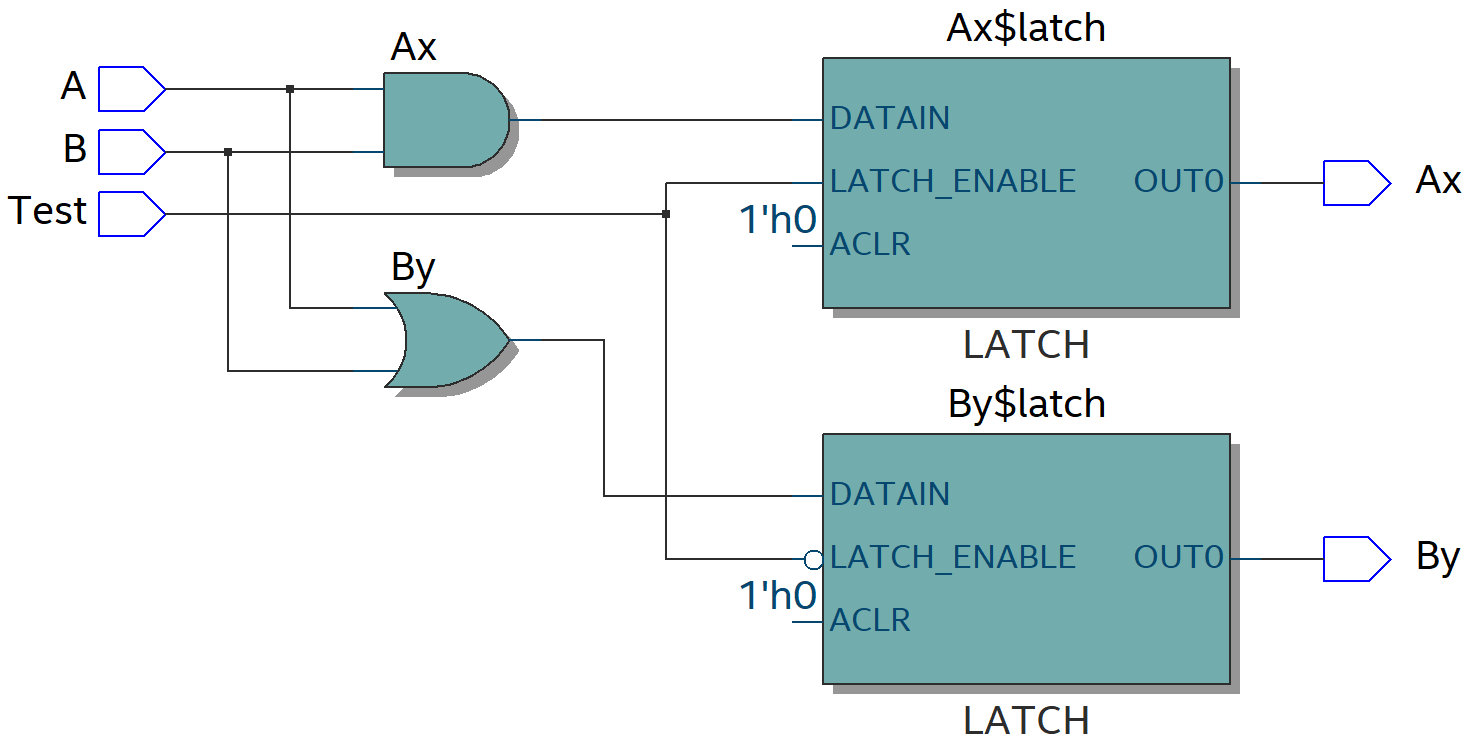
\includegraphics[scale=0.4]{Assignment_Circuit3_RTL.png}
	\caption{Diagrama RTL del circuito con estructura \textit{if-else}, descrito en Verilog. \label{fig:a_circuit3_rtl}}
\end{figure}

\begin{figure}[ht]
	\centering
	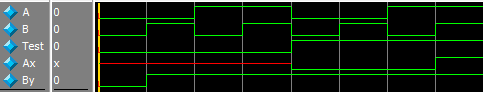
\includegraphics[scale=1.3]{Assignment_Circuit3_Wave.png}
	\caption{Simulación del circuito con estructura \textit{if-else}, descrito en Verilog, con el visor de formas de onda de ModelSim. \label{fig:a_circuit3_wave}}
\end{figure}